\documentclass[9pt]{beamer}
\usetheme[faculty=fi]{fibeamer}
\usepackage[T2A]{fontenc}
\usepackage[utf8]{inputenc}
\usepackage[
  main=ukrainian, %% By using `czech` or `slovak` as the main locale
                %% instead of `english`, you can typeset the
                %% presentation in either Czech or Slovak,
                %% respectively.
  english, russian %% The additional keys allow foreign texts to be
]{babel}        %% typeset as follows:
%%
%%   \begin{otherlanguage}{czech}   ... \end{otherlanguage}
%%   \begin{otherlanguage}{slovak}  ... \end{otherlanguage}
%%
%% These macros specify information about the presentation
\title{Криптосистеми на еліптичних кривих} %% that will be typeset on the
%\subtitle{Presentation Subtitle}
\subtitle{Lecture 2: Arithmetics}

\author{Грубіян Євген Олександрович}

%% These additional packages are used within the document:
\usepackage{ragged2e}  % `\justifying` text
\usepackage{booktabs}  % Tables
\usepackage{tabularx}
\usepackage{tikz}      % Diagrams
\usetikzlibrary{calc, shapes, backgrounds}
\usepackage{amsmath, amssymb}
\usepackage{url}       % `\url`s
\usepackage{listings}  % Code listings
\usepackage{wrapfig}
\frenchspacing
\begin{document}
  \frame{\maketitle}


  \begin{darkframes}
      
    \section{Light Frames}

\begin{frame}{Додавання двох точок на еліптичній кривій}
  \(P=(x_1,y_1), Q=(x_2,y_2), x_1\neq x_2\) --- точки на еліптичній кривій:
  \[
  E/K: \; y^2=x^3+ax+b, char(K) \neq 2,3
  \]

  \textbf{Крок 1.} Знаходимо нахил прямої $y=\lambda x + c$, що проходить через \(P\) та \(Q\):
  \[
  \lambda=\frac{y_2-y_1}{x_2-x_1}.
  \]

  \textbf{Крок 2.} Ця пряма перетинає нашу криву в 3х точках, координати яких задовольняють також рівняння кривої:
  \begin{align}
      & (\lambda x + c)^2 = x^3 + ax + b,\\
      & x^3 - (\lambda x + c)^2 + ax + b = 0
  \end{align}
  Оскільки $x_1, x_2, x_3$ координати точок є коренями одержаного поліному - коефіціент біля $x^2$ є сумою коренів зі зворотнім знаком за теоремою Вієта:
  $$
  \lambda^2 = x_1+x_2+x_3
  $$
  
\end{frame}

\begin{frame}{Додавання двох точок на еліптичній кривій}
    \textbf{Крок 3.} Оскільки сума будь яких трьох різних точок які є точками перетину довільної прямої та кривої визначається як $ P+Q+R=\mathcal{O}$, тоді $P+Q$ - відображення третьої точки \(R=(x_3,y_3)\) щодо осі \(x\), звідси отримуємо:

\begin{align}
    & R=-(P+Q)=(x_3,y_3) \\
    & x_3 = \lambda^2-x_1-x_2 \\
    & y_3=\lambda(x_3-x_1)+y_1.
\end{align}
Звідси:
$$
P+Q=-R=(x_3,-y_3)=(\lambda^2-x_1-x_2, \lambda(x_1-x_3)-y_1)
$$
Зауважимо також що операція додавання точок комутативна, що видно з симетричності формул додавання
\end{frame}
%%%%%%%%%%%%%%%%%%%%%%%%%%%%%%%%%%%%%%%%%%%%%%%%%%%%%%%%%%%%%%%%%%%%%%%%%%%%%%
% Слайд 2: Графічна ілюстрація додавання точок
%%%%%%%%%%%%%%%%%%%%%%%%%%%%%%%%%%%%%%%%%%%%%%%%%%%%%%%%%%%%%%%%%%%%%%%%%%%%%%
\begin{frame}{Графічна ілюстрація додавання точок в $\mathbb{E/R}$}
  \begin{center}
    \begin{tikzpicture}[scale=0.8]
      % Координатні осі
      \draw[->] (-2,0) -- (3,0) node[right] {\(x\)};
      \draw[->] (0,-2) -- (0,3) node[above] {\(y\)};
      
      % Еліптична крива: y^2 = x^3 - x.
      % Верхня гілка для x у [-1,0] та [1,3]
      \draw[domain=-1:0, smooth, variable=\x, red, thick] 
        plot ({\x}, {sqrt(\x*\x*\x - \x)});
      \draw[domain=1:2, smooth, variable=\x, red, thick] 
        plot ({\x}, {sqrt(\x*\x*\x - \x)});
      % Нижня гілка для x у [-1,0] та [1,3]
      \draw[domain=-1:0, smooth, variable=\x, red, thick] 
        plot ({\x}, {-sqrt(\x*\x*\x - \x)});
      \draw[domain=1:2, smooth, variable=\x, red, thick] 
        plot ({\x}, {-sqrt(\x*\x*\x - \x)});
      
      % Обчислення sqrt6
      \pgfmathsetmacro{\sqrtSix}{sqrt(6)}
      
      % Синя пряма: y = (\sqrt6/3)(x+1)
      \draw[domain=-1.5:2.5, smooth, variable=\x, blue, thick] 
        plot ({\x}, {(\sqrtSix/3)*(\x+1)});
      
      % Точка P = (-1, 0)
      \coordinate (P) at (-1,0);
      \fill (P) circle (2pt) node[below left] {\(P(-1,0)\)};
      
      % Точка Q = (2, \sqrt6)
      \coordinate (Q) at (2,{\sqrtSix});
      \fill (Q) circle (2pt) node[above right] {\(Q(2,\sqrt{6})\)};
      
      % Точка R = (-1/3, (2\sqrt6)/9) (на верхній гілці)
      \pgfmathsetmacro{\xR}{-1/3}
      \pgfmathsetmacro{\yR}{(2*\sqrtSix)/9}
      \coordinate (R) at (\xR,{\yR});
      \fill (R) circle (2pt) node[above left] {\(R\)};
      
      % Точка P+Q = відображення R через горизонтальну вісь: (-1/3, - (2\sqrt6)/9)
      \coordinate (S) at (\xR,{-\yR});
      \fill (S) circle (2pt) node[below left] {\(P+Q\)};
      
      % Провідна лінія для відображення точки R через горизонтальну вісь
      \draw[dashed] (R) -- (S);
    \end{tikzpicture}
  \end{center}
  \vspace{0.3cm}
  \footnotesize{Червоним нанесено еліптичну криву \(y^2=x^3-x\) над полем R. Синя пряма \(y=\frac{\sqrt{6}}{3}(x+1)\) проходить через точки \(P=(-1,0)\) та \(Q=(2,\sqrt{6})\) і перетинає криву в третій точці \(R=(-\frac{1}{3},\frac{2\sqrt{6}}{9})\). Відображення \(R\) через вісь \(x\) дає точку \(P+Q=(-\frac{1}{3},-\frac{2\sqrt{6}}{9})\).}
\end{frame}

%%%%%%%%%%%%%%%%%%%%%%%%%%%%%%%%%%%%%%%%%%%%%%%%%%%%%%%%%%%%%%%%%%%%%%%%%%%%%%
% Слайд 3: Подвоєння точки (виведення формул)
%%%%%%%%%%%%%%%%%%%%%%%%%%%%%%%%%%%%%%%%%%%%%%%%%%%%%%%%%%%%%%%%%%%%%%%%%%%%%%
\begin{frame}{Подвоєння точки на еліптичній кривій}
  Нехай \(P=(x_1,y_1)\) --- точка на \(E/K: \; y^2=x^3+ax+b\) з \(y_1\neq 0\).

  \bigskip
  \textbf{Крок 1.} Знаходимо нахил дотичної до \(E\) в точці \(P\):
  \[
  \lambda=\frac{dy}{dx}=\frac{3x_1^2+a}{2y_1}.
  \]

  \textbf{Крок 2.} Дотична перетинає криву ще в одній точці $R=(x_3,y_3)$, тому за аналогією:
  \begin{align}
  & x_3=\lambda^2-2x_1\\
  & y_3=\lambda(x_3-x_1)+y_1.
  \end{align}

  Таким чином, подвоєння точки задається формулою:
  \[
  2P=(x_3,-y_3)=(\lambda^2-2x_1, \lambda (x_1-x_3)-y_1)
  \]
\end{frame}

%%%%%%%%%%%%%%%%%%%%%%%%%%%%%%%%%%%%%%%%%%%%%%%%%%%%%%%%%%%%%%%%%%%%%%%%%%%%%%
% Слайд 4: Графічна ілюстрація подвоєння точки
%%%%%%%%%%%%%%%%%%%%%%%%%%%%%%%%%%%%%%%%%%%%%%%%%%%%%%%%%%%%%%%%%%%%%%%%%%%%%%
\begin{frame}{Графічна ілюстрація подвоєння точки в $\mathbb{E/R}$}
  \begin{center}
    \begin{tikzpicture}[scale=0.8]
      % Координатні осі
      \draw[->] (-2,0) -- (3,0) node[right] {\(x\)};
      \draw[->] (0,-2) -- (0,3) node[above] {\(y\)};
      
      % Еліптична крива: y^2 = x^3 - x.
      % Ліва частина (x від -1 до 0)
      \draw[domain=-1:0, smooth, variable=\x, red, thick] 
        plot ({\x}, {sqrt(max(0,\x*\x*\x - \x))});
      \draw[domain=-1:0, smooth, variable=\x, red, thick] 
        plot ({\x}, {-sqrt(max(0,\x*\x*\x - \x))});
      % Права частина (x від 1 до 2.5)
      \draw[domain=1:2, smooth, variable=\x, red, thick] 
        plot ({\x}, {sqrt(\x*\x*\x - \x)});
      \draw[domain=1:2, smooth, variable=\x, red, thick] 
        plot ({\x}, {-sqrt(\x*\x*\x - \x)});
      
      % Задаємо точку P з лівої гілки:
      % P = (-0.5, sqrt(3/8))
      \pgfmathsetmacro{\xP}{-0.5}
      \pgfmathsetmacro{\yP}{sqrt(3/8)}
      \coordinate (P) at (\xP,{\yP});
      \fill (P) circle (2pt) node[above left] {\(P(-0.5,\sqrt{3/8})\)};
      
      % Обчислюємо нахил дотичної в P:
      % m = (3*x_P^2 - 1)/(2*y_P)
      \pgfmathsetmacro{\m}{(3*(\xP*\xP)-1)/(2*\yP)}
      
      % Наносимо дотичну в точці P: рівняння y = m*(x - x_P) + y_P
      \draw[blue, thick, domain=-1.5:2.5] 
        plot (\x, {\m*(\x - \xP) + \yP});
      
      % Обчислюємо координату точки R:
      % x_R = m^2 - 2*x_P
      \pgfmathsetmacro{\xR}{\m*\m - 2*\xP}
      % y_R = m*(x_P - x_R) - y_P
      \pgfmathsetmacro{\yR}{\m*(\xP - \xR) - \yP}
      
      \coordinate (R) at (\xR,{\yR});
      \fill (R) circle (2pt) node[below right] {\(2P\)};
      
      % Точка 2P = (x_R, -y_R)
      \coordinate (TwoP) at (\xR,{-\yR});
      \fill (TwoP) circle (2pt) node[below right] {\(R(x_3,y_3)\)};
      
      % Провідна лінія, що показує відображення R через ось x (заміна знака y)
      \draw[dashed] (R) -- (TwoP);
    \end{tikzpicture}
  \end{center}
  \vspace{0.3cm}
  \footnotesize{Червоним нанесено еліптичну криву \(y^2=x^3-x\) над R. Синя дотична в точці \(P(-0.5,\sqrt{3/8})\) перетинає криву в точці \(R(x_3,y_3)\); відображення \(R\) через горизонтальну вісь дає \(2P=(x_3,-y_3)\).}
\end{frame}


% Слайд 1: Тема лекції
\begin{frame}{Скалярний добуток та порядок точки}
  Часто в криптографії використовують так звану операцію скалярного добутку:
  $$Q=[k]P$$
  Що означає додати точку $P$ саму до себе $k$ разів
  \begin{block}{Порядок точки $ord(P)$}
      Таке мінімальне число $n \in \mathbb{N}_0$ що $[n]P=\mathcal{O}$ або $0$ якщо такого натурального числа не існує.
  \end{block}
\end{frame}

\begin{frame}{Проективна площина}
  \begin{block}{Проективна площина $\mathbb{P}^2(K)$ над полем $K$}
    \[
    \mathbb{P}^2(K) = \{(X:Y:Z) \in K^3 \setminus \{(0,0,0)\}\} \big/ \sim,
    \]
    де еквівалентність задана співвідношенням
    \[
    \exists \lambda\in K^\times \quad (X:Y:Z) \sim (\lambda X:\lambda Y:\lambda Z)
    \]
  \end{block}
  \begin{block}{Перехід між афінними та проективними координатами}
    \begin{align}
        & (X:Y:Z) \xrightarrow{aff} (X/Z, Y/Z) \\
        & (x,y) \xrightarrow{proj} (x: y: 1)
    \end{align}
  \end{block}
\end{frame}

% Слайд 2: Проективні координати
\begin{frame}{Проективні координати}
Еліптичні криві зручно задавати в проективних координатах, оскільки реалізація арифметики значно ефективніша через відсутність "дорогого" ділення в полі

  \begin{block}{Еліптична крива над полем $K, char(K) \neq 2,3$}
  Множина точок $P = (X:Y:Z) \in \mathbb{P}^2(\overline{K})$, що задовольняють рівнянню Вейєрштраса:
  \[
  E_{\mathbb{P}}/K: Y^2Z = X^3 + aXZ^2 + bZ^3,\quad a,b\in K,\quad \Delta = 4a^3+27b^2\neq 0.
  \]

\end{block}
  Зазначимо, що точка на нескінченності перейде в $\mathcal{O} \xrightarrow{proj} (0:1:0)$
\end{frame}

% Слайд 4: Формули додавання в проективних координатах
\begin{frame}{Формули додавання в проективних координатах}
  Нехай \(P=(X_1:Y_1:Z_1)\) та \(Q=(X_2:Y_2:Z_2)\) --- точки на еліптичній кривій, заданій рівнянням
  \[
  Y^2Z = X^3 + aXZ^2 + bZ^3.
  \]
  \textbf{Визначимо проміжні змінні:}
  \[
  \begin{aligned}
  U_1 &= Y_1 Z_2,\quad &U_2 &= Y_2 Z_1,&
  V_1 &= X_1 Z_2,\quad &V_2 &= X_2 Z_1,\\
  U &= U_2 - U_1,\quad &V &= V_2 - V_1.
  \end{aligned}
  \]
  При умові \(V\neq 0\) координати суми \(P+Q=(X_3:Y_3:Z_3)\) можна записати як:
  \[
  \begin{aligned}
  X_3 &= U^2Z_1Z_2 - V^3 - 2V^2V_1,\\[1mm]
  Y_3 &= U\Bigl(V^3 + 2V^2V_1 - X_3V_1\Bigr) - V^3U_1,\\[1mm]
  Z_3 &= V^3Z_1Z_2.
  \end{aligned}
  \]
\end{frame}

\begin{frame}{Формули додавання в проективних координатах (спеціальні випадки)}
  \textbf{1. Подвоєння точки (коли \(P=Q\)):} \\
  Нехай \(P=(X_1:Y_1:Z_1)\) — точка еліптичної кривої
  \[
  Y^2Z = X^3 + aXZ^2 + bZ^3.
  \]
  Визначимо:
  \[
  \begin{array}{aligned}
  W = 3X_1^2 + aZ_1^2,&
  S = Y_1Z_1,&
  B = X_1Y_1,&
  H = W^2 - 8B,\\
  X_3 = 2S\,H,&
  Y_3 = W(4B - H) - 8Y_1^2X_1,&
  Z_3 = 8S^3.
  \end{array}
  \]
  Тоді подвоєння точки записується як:
  \[
  2P = (X_3:Y_3:Z_3).
  \]
  
  \vspace{0.5cm}
  \textbf{2. Якщо \(Q=-P\), тобто}
  $
  Q=(X_1:-Y_1:Z_1)
  $
  то
  $
  P + (-P) = \mathcal{O},
  $

\end{frame}


% Слайд 3: Означення еліптичної кривої
\begin{frame}{Ілюстрація еліптичної кривої в проективній площині}
    \begin{center}
    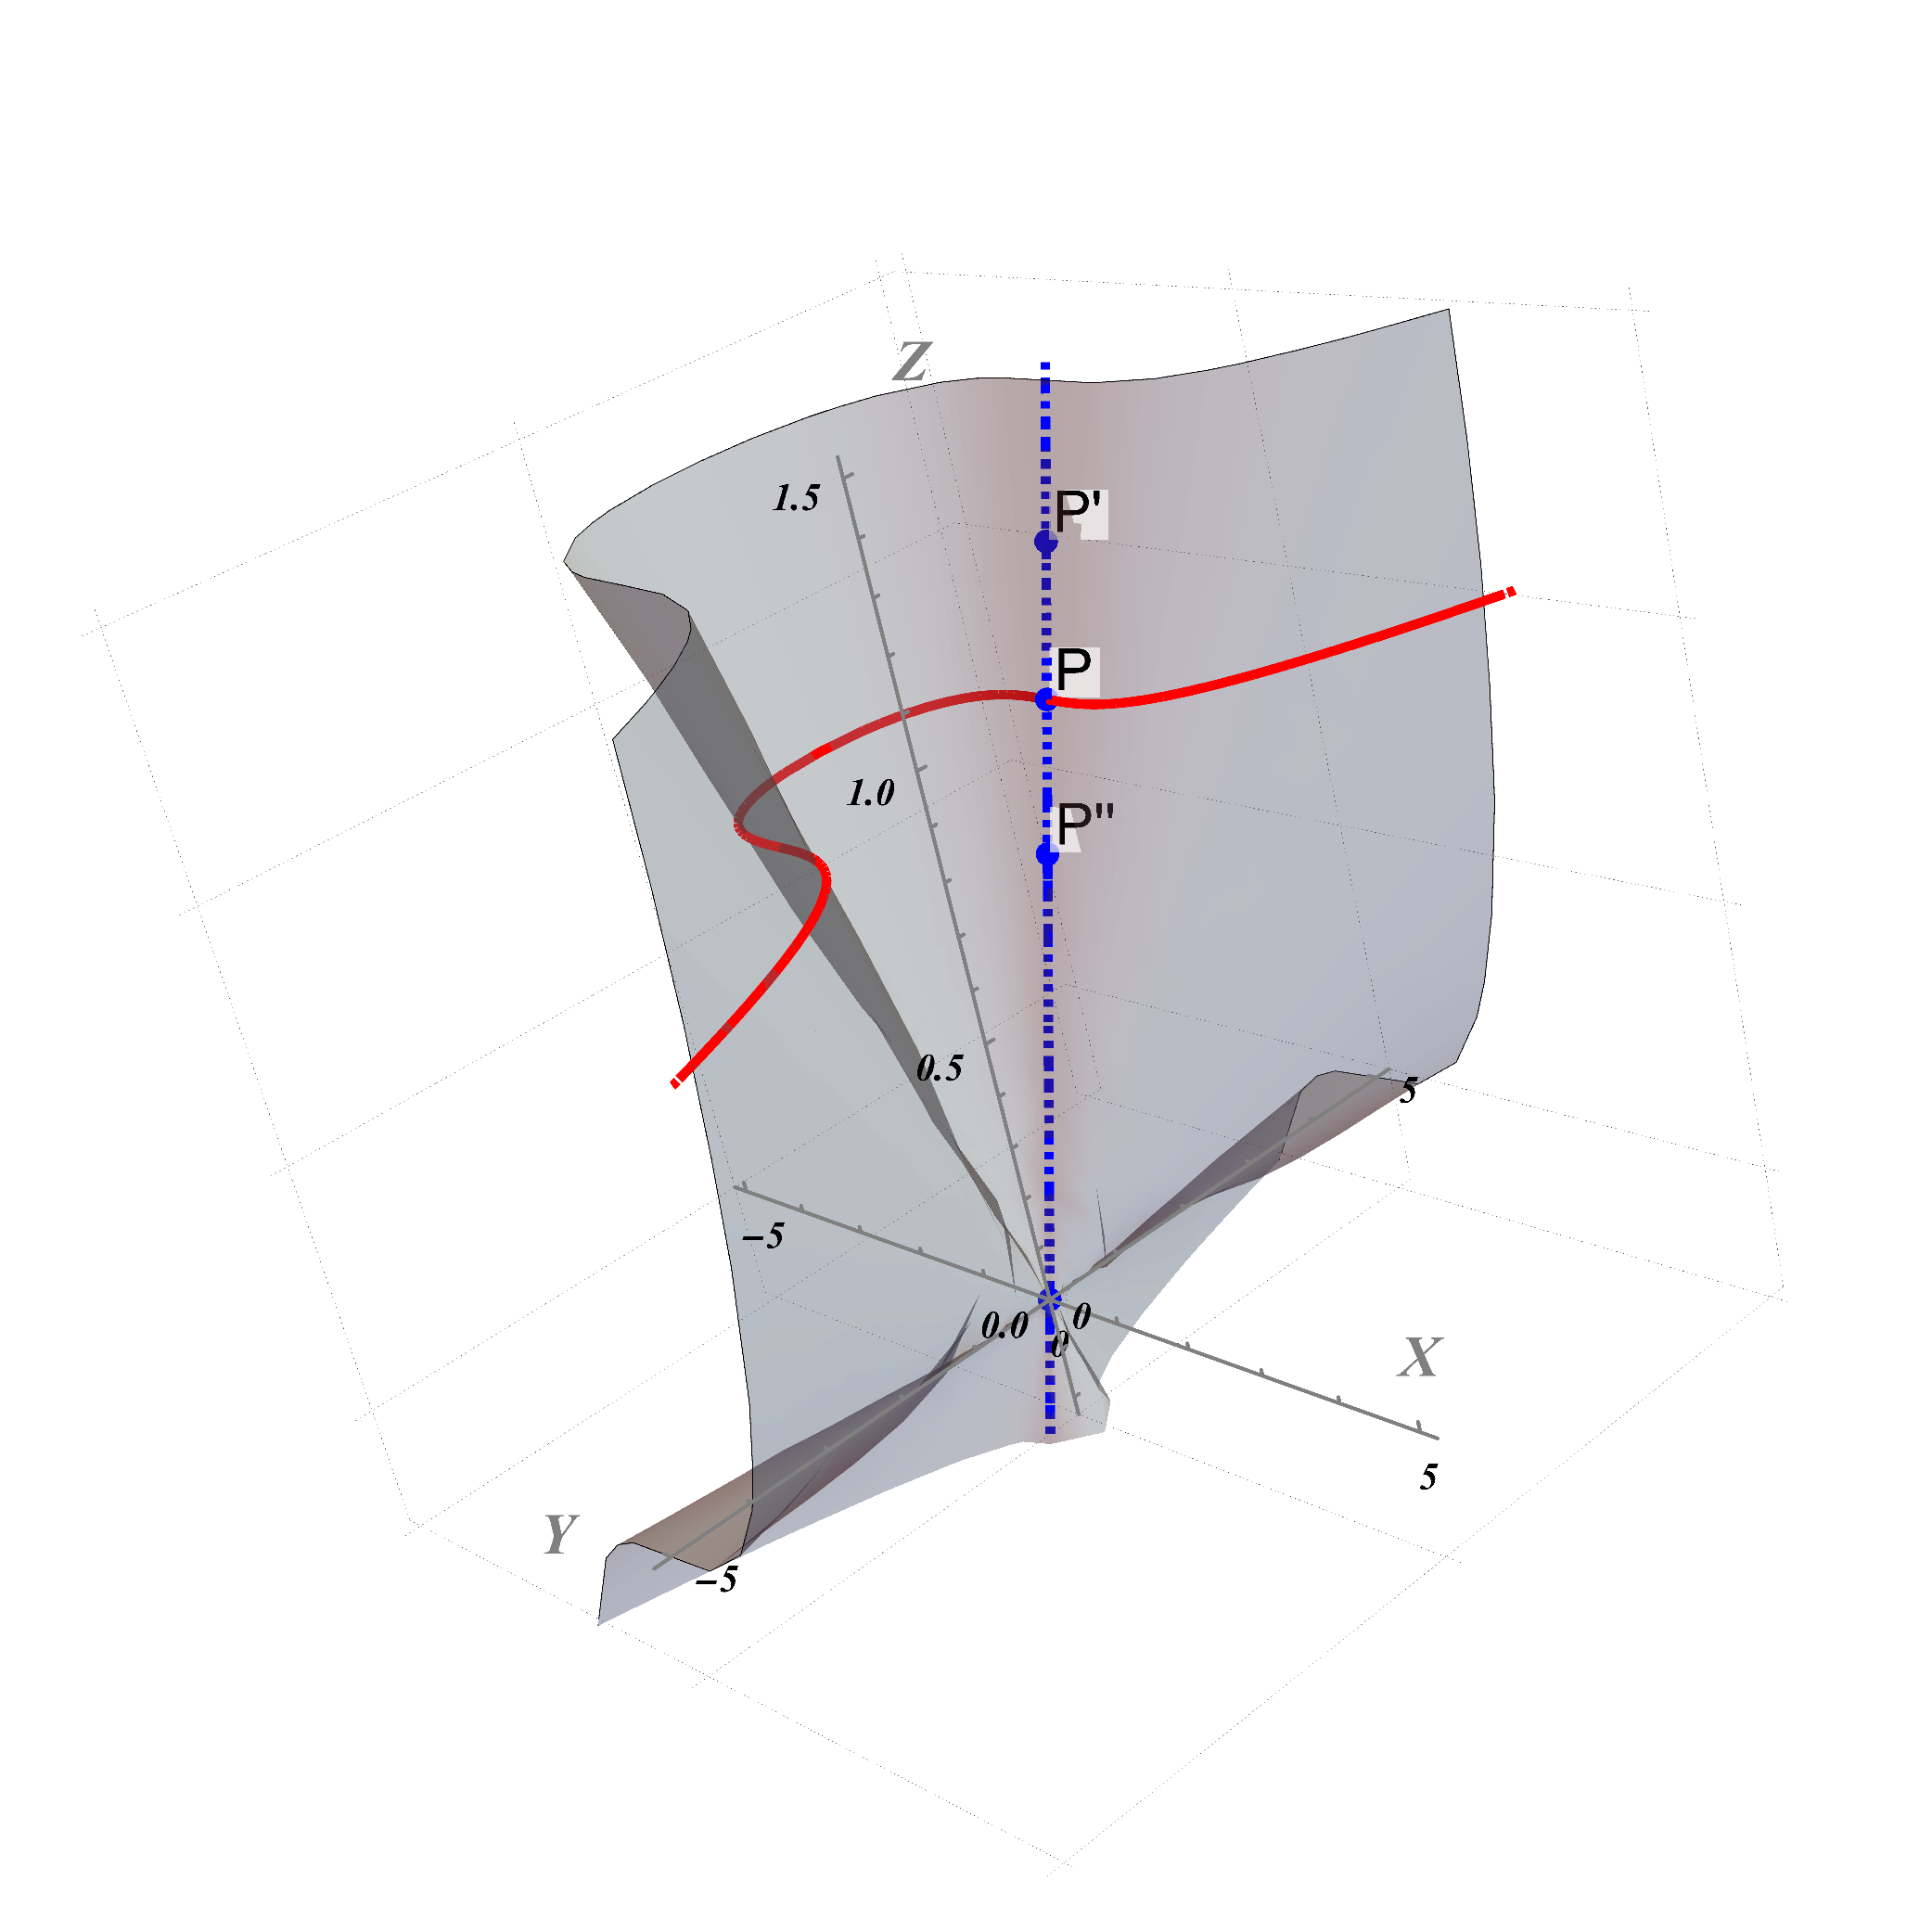
\includegraphics[width=0.9\textwidth]{resources/projective_ec.pdf}
    \end{center}
\end{frame}


  \end{darkframes}




\end{document}
